%% Supplementary material (SI.pdf) for the Review of Scientific Instruments
%% manuscript (paper.tex).
%%
%% Format follows the AIP Publishing author instructions ("Using Supplementary
%% Material in Your Manuscript", mirrored in
%% template/rsi/aip-author-instructions-2026-07-02.txt):
%%   - at initial submission, supplementary material is uploaded as a single
%%     separate PDF named SI.pdf;
%%   - supplementary figures/tables carry S-prefixed numbers (Fig. S1, Table S1);
%%   - alt text is included under each figure/table caption in the SI file;
%%   - after acceptance AIP deposits the file in Figshare with its own DOI.
%%
%% Content is compiled from the version-controlled sources in
%% paper/supplementary/ (supplementary-figures.md, specimen-run-linkage.md,
%% bill-of-materials.md, design-file-inventory.md); those files remain the
%% editable sources of record. Build: `make si` (pdflatex x2).
%%
\documentclass[10pt,letterpaper]{article}

\usepackage[margin=2.2cm]{geometry}
\usepackage{graphicx}
\usepackage{booktabs}
\usepackage{array}
\usepackage{tabularx}
\usepackage{pdflscape}
\usepackage{textcomp}
\usepackage{xcolor}
\usepackage[colorlinks=true,allcolors=blue]{hyperref}
\usepackage[htt]{hyphenat} % allow long \texttt{} paths to break across lines
\sloppy

% S-prefixed numbering per AIP supplementary-material convention.
\renewcommand{\thefigure}{S\arabic{figure}}
\renewcommand{\thetable}{S\arabic{table}}
\renewcommand{\thesection}{S\Roman{section}}
\renewcommand{\thesubsection}{\thesection.\Alph{subsection}}

\newcommand{\dC}{\,$^{\circ}$C}
\newcommand{\um}{\,\textmu m}
% Alt text under each caption (AIP accessibility instructions for SI files).
\newcommand{\alttext}[1]{\par\smallskip{\footnotesize\emph{Alt text:} #1\par}}
% Hyperlink a run ID to its raw log in the data repository.
\newcommand{\runlog}[2]{\href{https://github.com/vertical-cloud-lab/custom-induction-furnace/blob/main/docs/data_log/#1}{#2}}

\newcolumntype{L}[1]{>{\raggedright\arraybackslash}p{#1}}

\begin{document}

\begin{center}
{\Large\bfseries Supplementary material for:\\[2pt]
Retrofitting a commercial RF induction generator into a computer-controlled,
vacuum-integrated annealing system for reactive-metal grain growth}\\[10pt]
Sterling G. Baird, Ryan Weber, Christopher Nyborg, Ronnie Guymon,
Gage Erickson, and Oliver Johnson\\[2pt]
{\itshape Department of Mechanical Engineering, Brigham Young University,
Provo, Utah 84602, USA}
\end{center}

\medskip
\noindent This document collects the supplementary figures
(Figs.~S1--S13), the specimen--thermal-history linkage
(Table~\ref{tab:linkage}), the itemized bill of materials
(Table~\ref{tab:bom}), and the design-file inventory
(Table~\ref{tab:designfiles}) that support the main text. File paths are
relative to the root of the openly available data and design repository
(\url{https://github.com/vertical-cloud-lab/custom-induction-furnace}); an
archival snapshot is deposited at Zenodo,
\href{https://doi.org/10.5281/zenodo.20878017}{10.5281/zenodo.20878017}. All
plotted figures are rendered reproducibly from the raw logs by the
\texttt{paper/build\_*.py} scripts (\texttt{make figures}); the data figures
in the main text are the laboratory's actual recorded images, extracted
verbatim. Alt text is provided under each figure and table caption per the
AIP Publishing accessibility instructions.

%==============================================================
\section{Hardware}
%==============================================================

\begin{figure}[htbp]
\centering
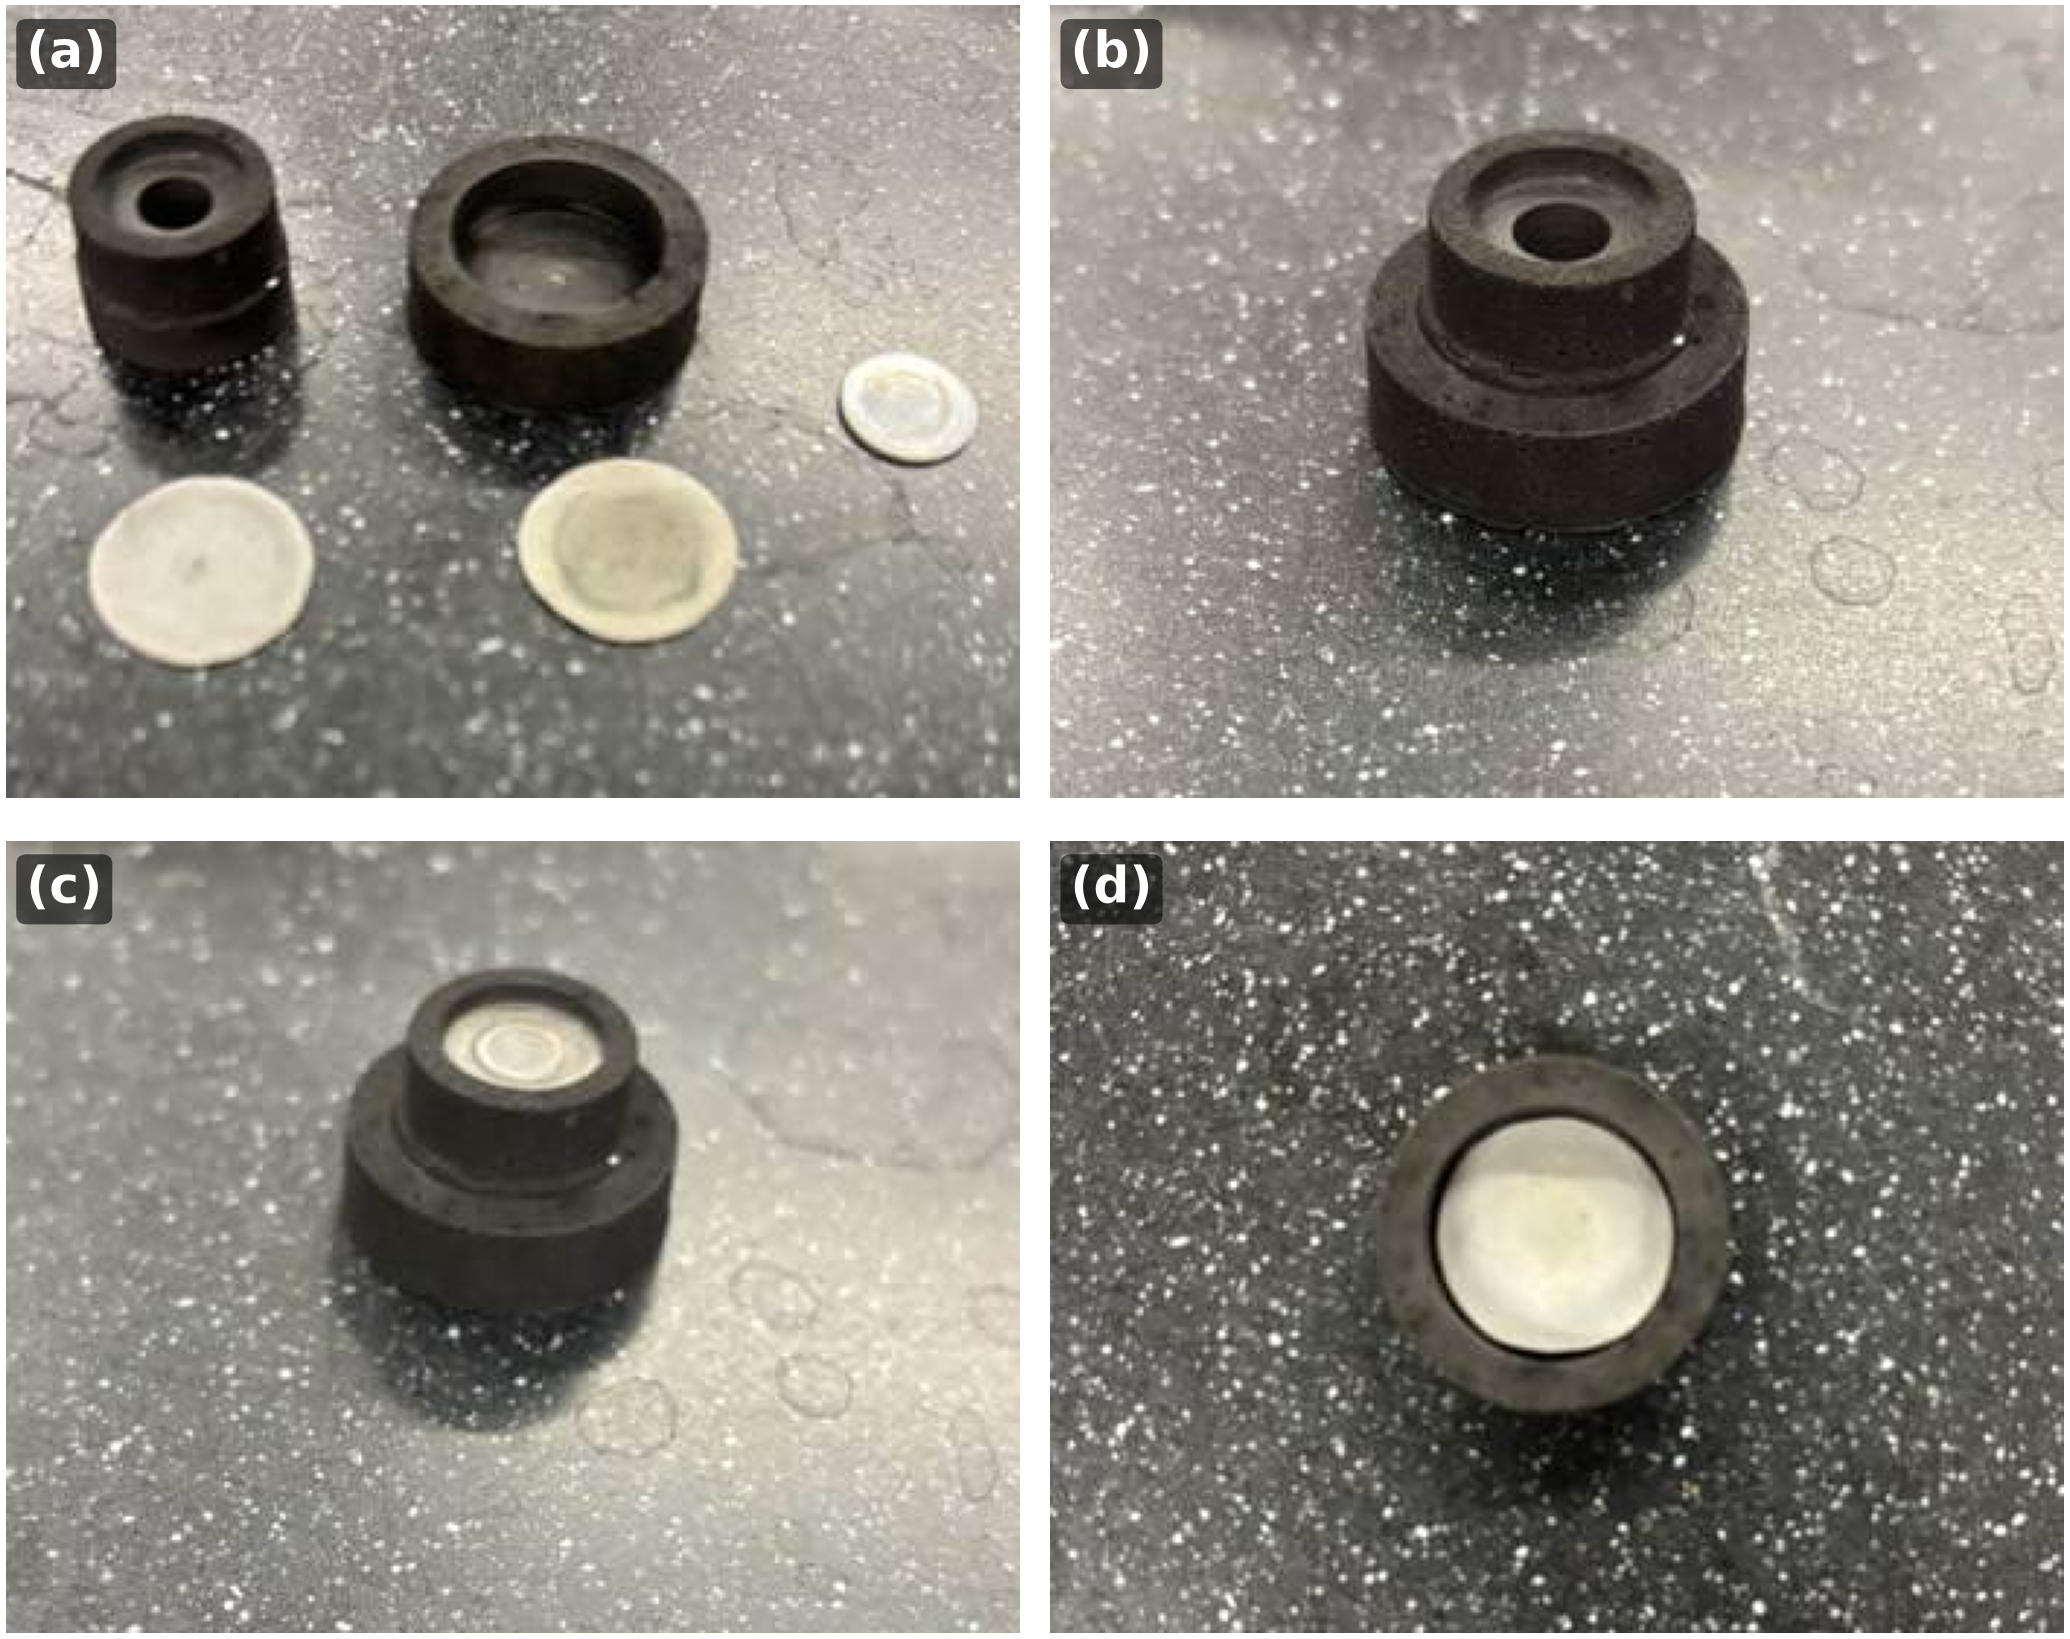
\includegraphics[width=0.55\linewidth]{figures/fig_crucible.png}
\caption{Fully disassembled graphite crucible. Top left is the crucible lid,
top middle is the bottom of the crucible that acts as the specimen carrier,
far right is the sapphire window, bottom left and middle are the alumina
sample-surrounding sheets.}
\label{fig:s-crucible}
\alttext{Photograph of the disassembled graphite crucible parts: a stepped
lid, the cup-shaped specimen carrier, a small transparent sapphire window
disc, and two thin white alumina sheets.}
\end{figure}

\begin{figure}[htbp]
\centering
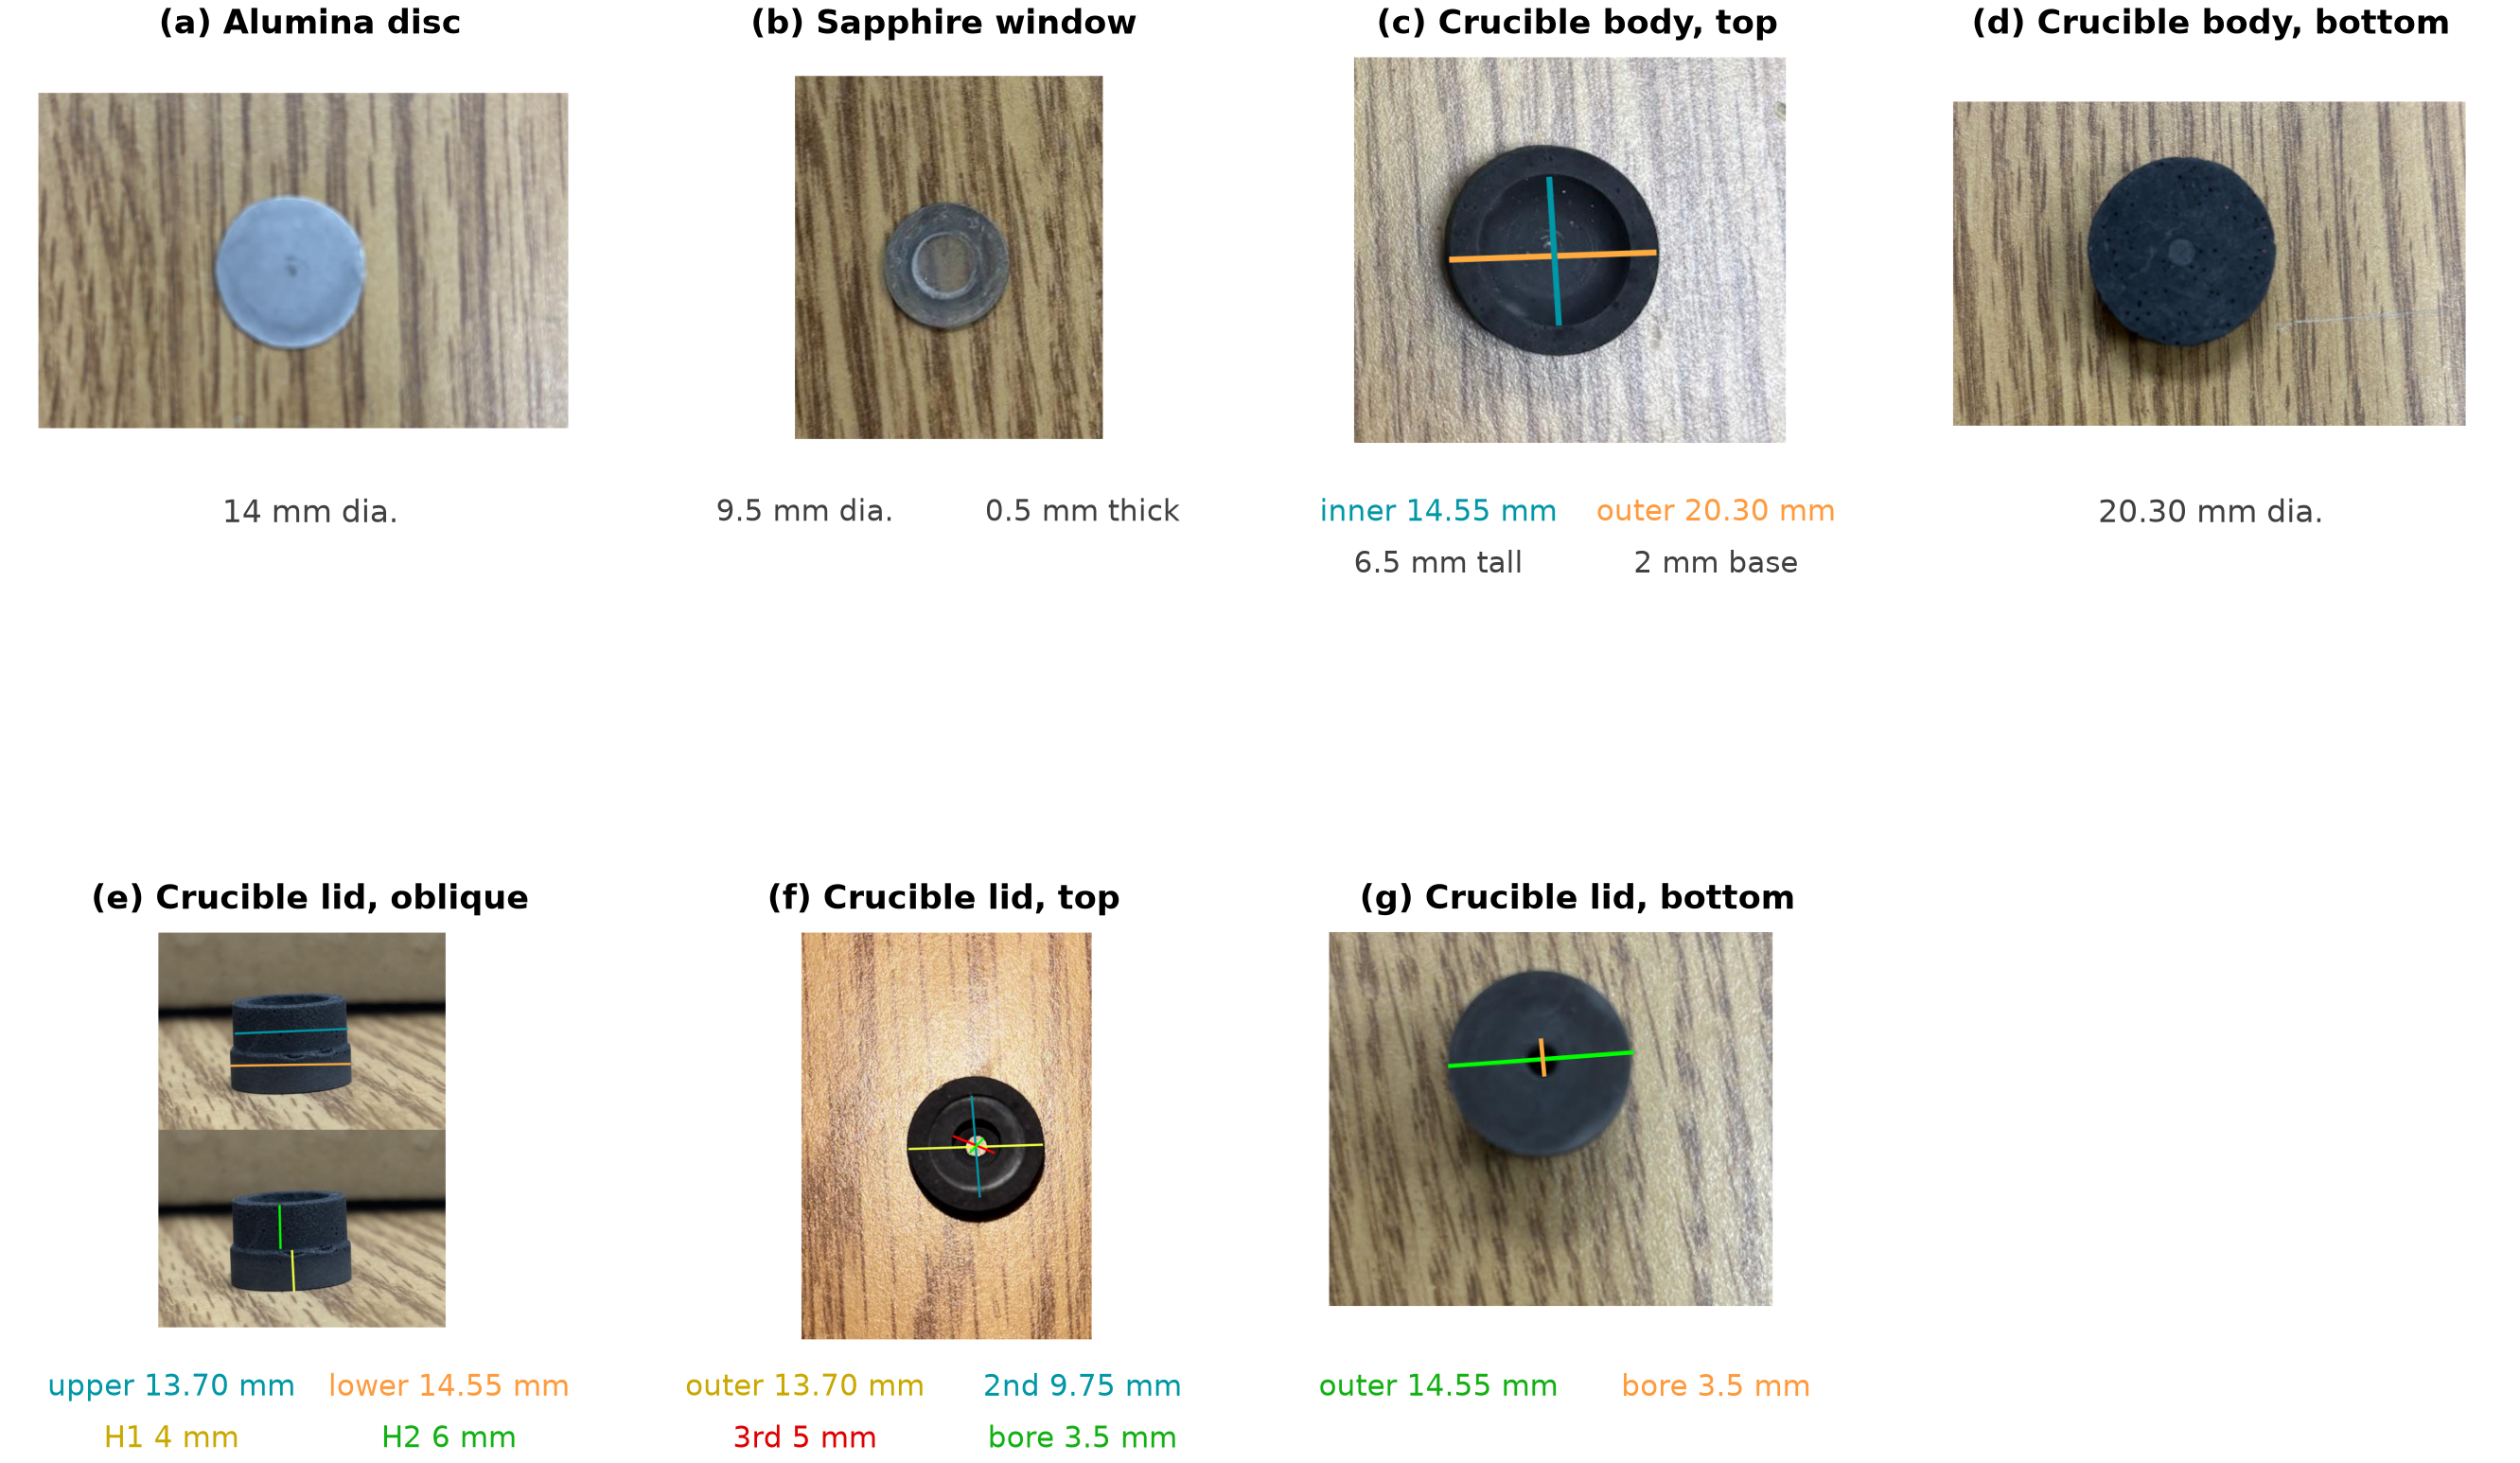
\includegraphics[width=0.9\linewidth]{figures/fig_crucible_dimensions.png}
\caption{Measured dimensions of each part of the graphite crucible/susceptor
stack, with the coloured measurement lines drawn on the corresponding
photograph. (a)~Alumina spacer disc, 14\,mm dia. (b)~Sapphire pyrometer
window, 9.5\,mm dia., 0.5\,mm thick. (c)~Crucible body, top: machined sample
cavity 14.55\,mm ID (teal), 20.30\,mm OD (orange); the cup is 6.5\,mm tall
with a 2\,mm base. (d)~Crucible body, bottom face, 20.30\,mm dia.
(e)~Crucible lid, oblique: the stepped plug seats into the cavity ---
13.70\,mm upper step (teal), 14.55\,mm lower shoulder (orange); the upper
step is 4\,mm tall (H1, yellow) and the lower shoulder 6\,mm tall (H2,
green). (f)~Crucible lid, top: four concentric steps of 13.70\,mm
(outermost), 9.75\,mm, 5\,mm, and a 3.5\,mm central pyrometer-sighting bore.
(g)~Crucible lid, bottom: 14.55\,mm seating face (green) and the 3.5\,mm
through-bore (orange). Fully assembled the stack stands 13\,mm tall.}
\label{fig:s-crucible-dims}
\alttext{Seven labeled photographs of the crucible parts, each overlaid with
colored measurement lines and numeric callouts giving the diameters, step
heights, and the central pyrometer bore dimensions.}
\end{figure}

\begin{figure}[htbp]
\centering
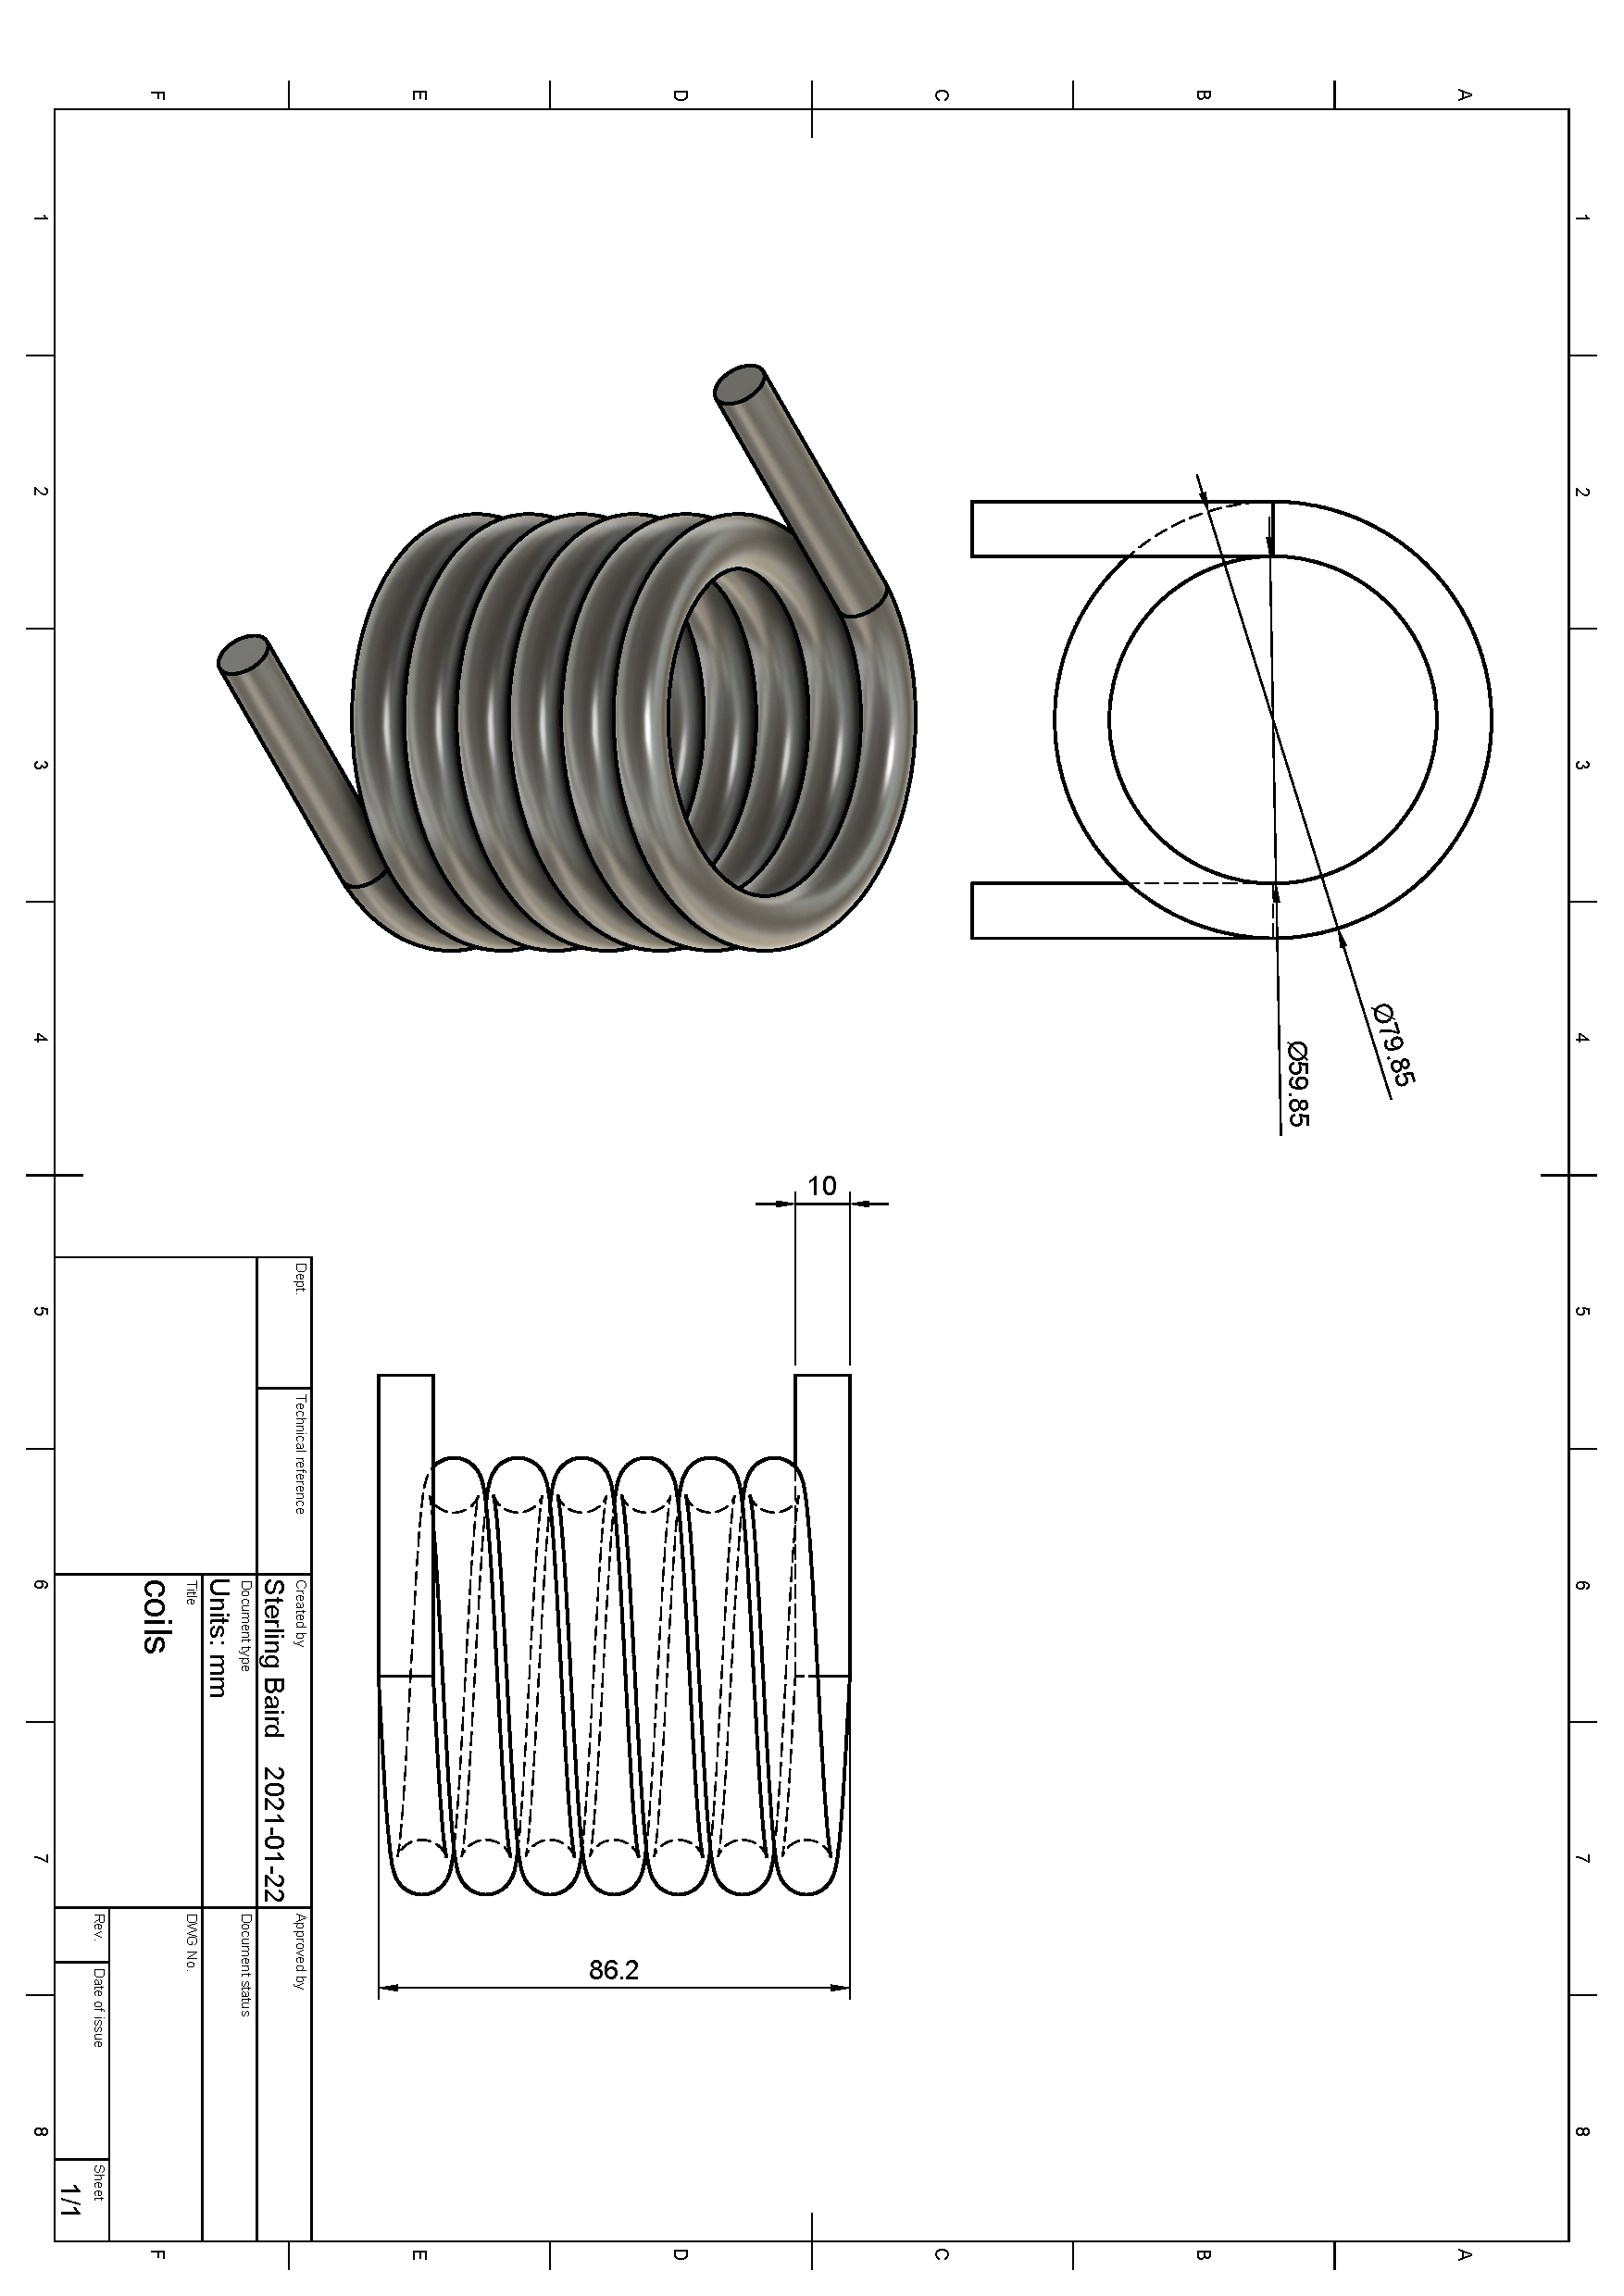
\includegraphics[width=0.62\linewidth]{../docs/coils-drawing.pdf}
\caption{Work-coil fabrication drawing used for the current build, showing
the coil geometry and dimensional callouts used to form and mount the
liquid-cooled copper coil around the quartz chamber. (Source file:
\texttt{docs/coils-drawing.pdf}.)}
\label{fig:s-coil}
\alttext{Engineering drawing of the liquid-cooled copper work coil with
dimensional callouts for the coil height, inner diameter, number of turns,
and lead routing.}
\end{figure}

\begin{figure}[htbp]
\centering
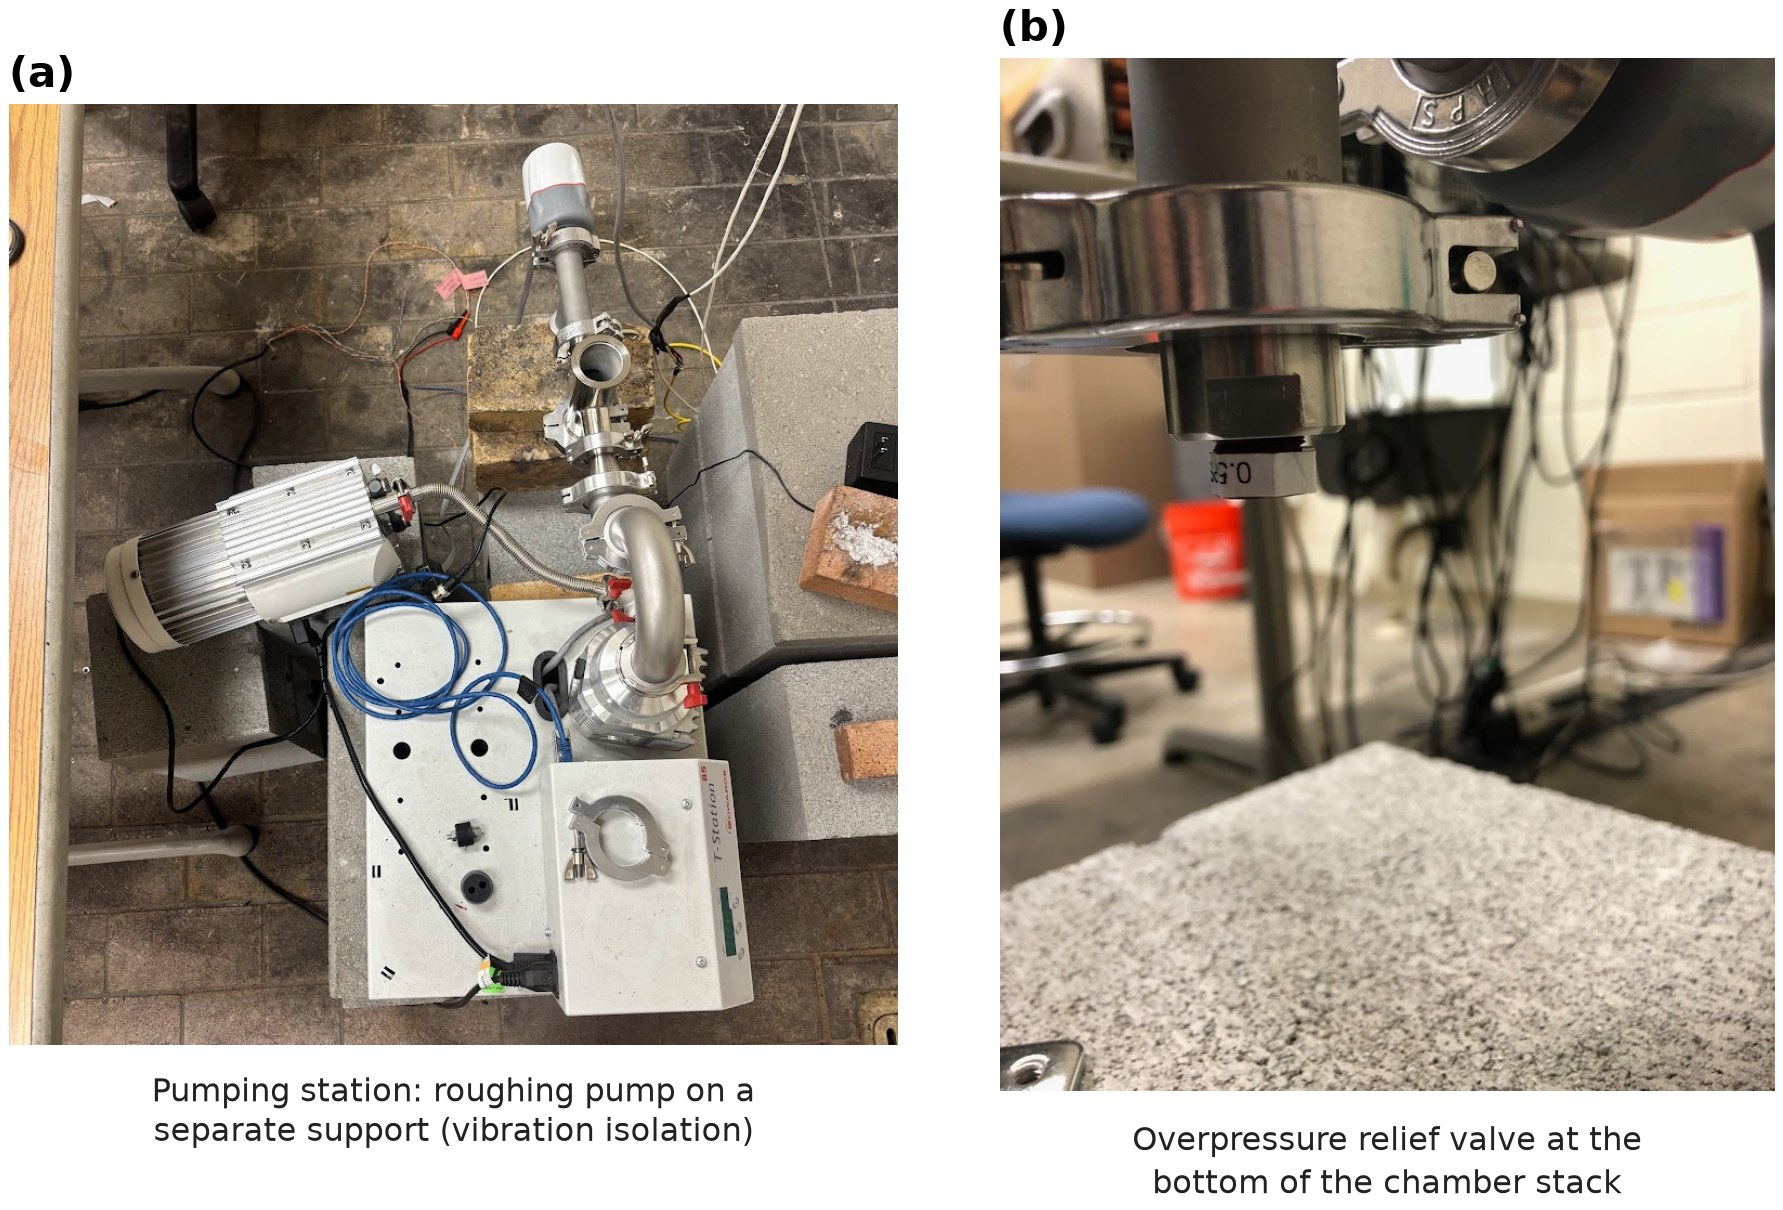
\includegraphics[width=0.72\linewidth]{figures/fig_vacuum_details.jpg}
\caption{Vacuum and gas-handling details. (a)~Turbo pumping station with the
roughing pump mounted on a separate support, coupled to the pumping station
only through a flexible hose, so pump vibration is not transmitted into the
chamber. (b)~Overpressure relief valve (0.5\,psi cracking pressure) at the
bottom of the vacuum chamber stack.}
\label{fig:s-vacuum}
\alttext{Two photographs: a turbo pumping station beside a separately
supported roughing pump joined only by a flexible hose, and a small brass
relief valve fitted at the base of the chamber stack.}
\end{figure}

\clearpage
%==============================================================
\section{Thermal performance}
%==============================================================

\begin{figure}[htbp]
\centering
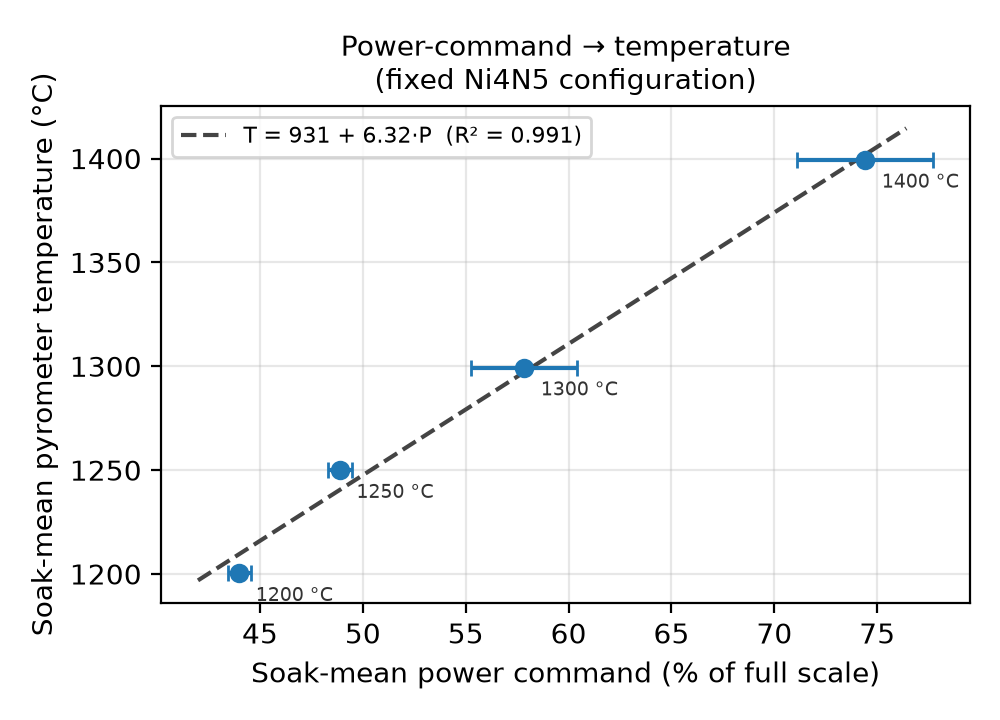
\includegraphics[width=0.6\linewidth]{figures/fig_calibration.png}
\caption{Power-command\,$\rightarrow$\,temperature calibration for one fixed
Ni4N5 configuration. Points are soak-mean values; horizontal bars are the
in-soak standard deviation of the analog command. The dashed line is the
linear operational calibration ($R^2 = 0.991$, $n = 4$).}
\label{fig:s-calibration}
\alttext{Scatter plot of soak-mean temperature against analog power command
with four points between 1200 and 1400 degrees Celsius and a dashed straight
fit line through them.}
\end{figure}

\begin{figure}[htbp]
\centering
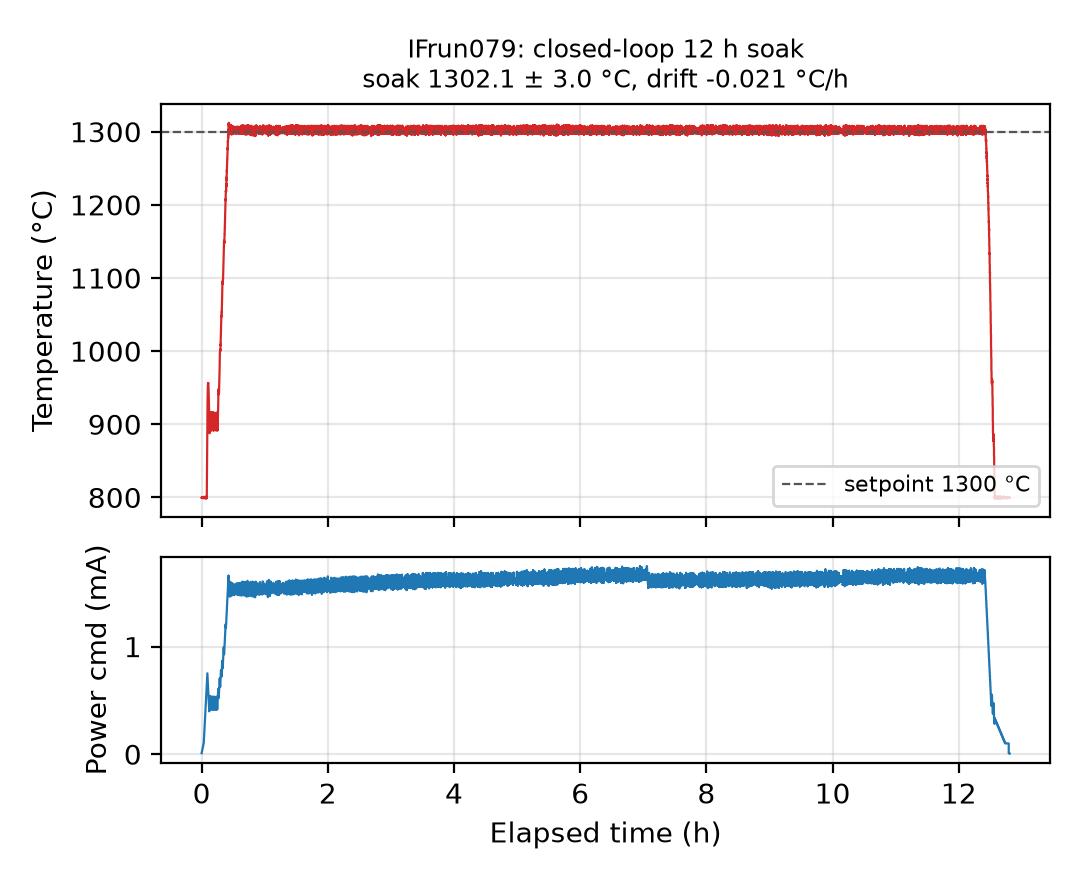
\includegraphics[width=0.6\linewidth]{figures/fig_representative.png}
\caption{Representative closed-loop anneal (Ni4N5, nominal
1300\dC{} / 12\,h): pyrometer temperature with setpoint overlay (top) and
analog power command (bottom). Soak mean $1302.1 \pm 3.0$\dC, drift
$-0.02$\dC/h.}
\label{fig:s-representative}
\alttext{Two stacked line plots over twelve hours: the pyrometer temperature
rising to and holding near 1300 degrees Celsius on its setpoint, and the
analog power command settling to a steady value below.}
\end{figure}

\begin{figure}[htbp]
\centering
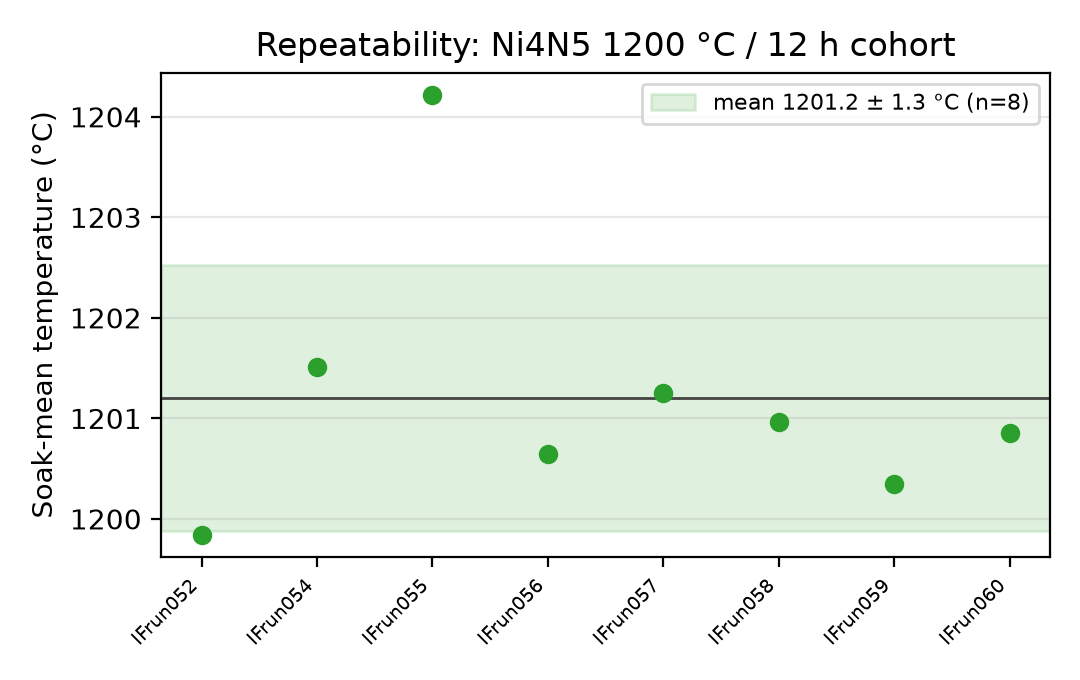
\includegraphics[width=0.6\linewidth]{figures/fig_repeatability.png}
\caption{Repeatability of the Ni4N5 1200\dC{} / 12\,h cohort ($n = 8$).
Points are per-run soak-mean temperatures; the band is
mean\,$\pm$\,SD ($1201.2 \pm 1.3$\dC).}
\label{fig:s-repeatability}
\alttext{Plot of eight per-run soak-mean temperatures clustered near 1200
degrees Celsius inside a shaded band marking the mean plus or minus one
standard deviation.}
\end{figure}

\begin{figure}[htbp]
\centering
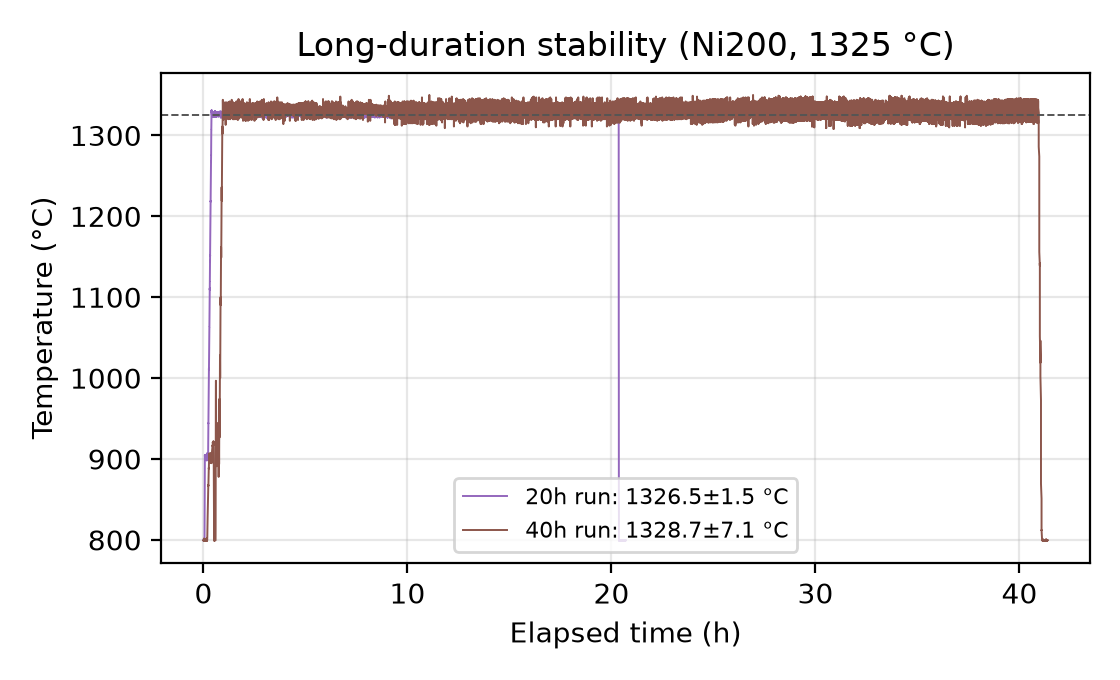
\includegraphics[width=0.6\linewidth]{figures/fig_longsoak.png}
\caption{Long-duration thermal stability: Ni200 anneals at 1325\dC{} held
for 20\,h and 40\,h.}
\label{fig:s-longsoak}
\alttext{Line plot of two anneal temperature traces at 1325 degrees Celsius,
one held twenty hours and one held forty hours, both essentially flat across
the soak.}
\end{figure}

\clearpage
%==============================================================
\section{Microstructure}
%==============================================================

\begin{figure}[htbp]
\centering
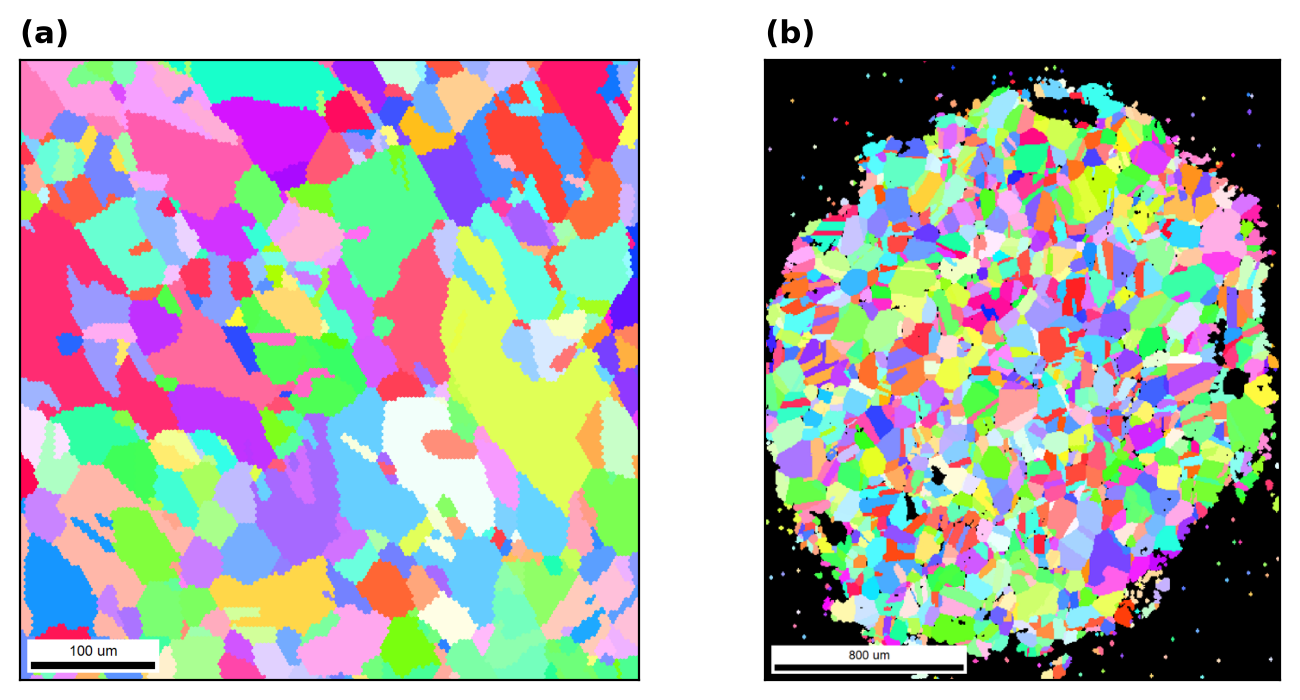
\includegraphics[width=0.72\linewidth]{figures/fig_ebsd.png}
\caption{EBSD inverse-pole-figure (IPF) orientation maps of two annealed
Ni4N5 specimens, rendered from the recorded EBSD scans.
(a)~Ni4N5\_034 (annealed at 1200\dC{} / 12\,h); (b)~Ni4N5\_069. Each indexed
color is a crystallographic orientation; the maps resolve hundreds of grains
for grain-size and texture analysis.}
\label{fig:s-ebsd}
\alttext{Two colorful electron-backscatter-diffraction orientation maps in
which each colored patch is a differently oriented grain, together resolving
hundreds of grains.}
\end{figure}

\begin{figure}[htbp]
\centering
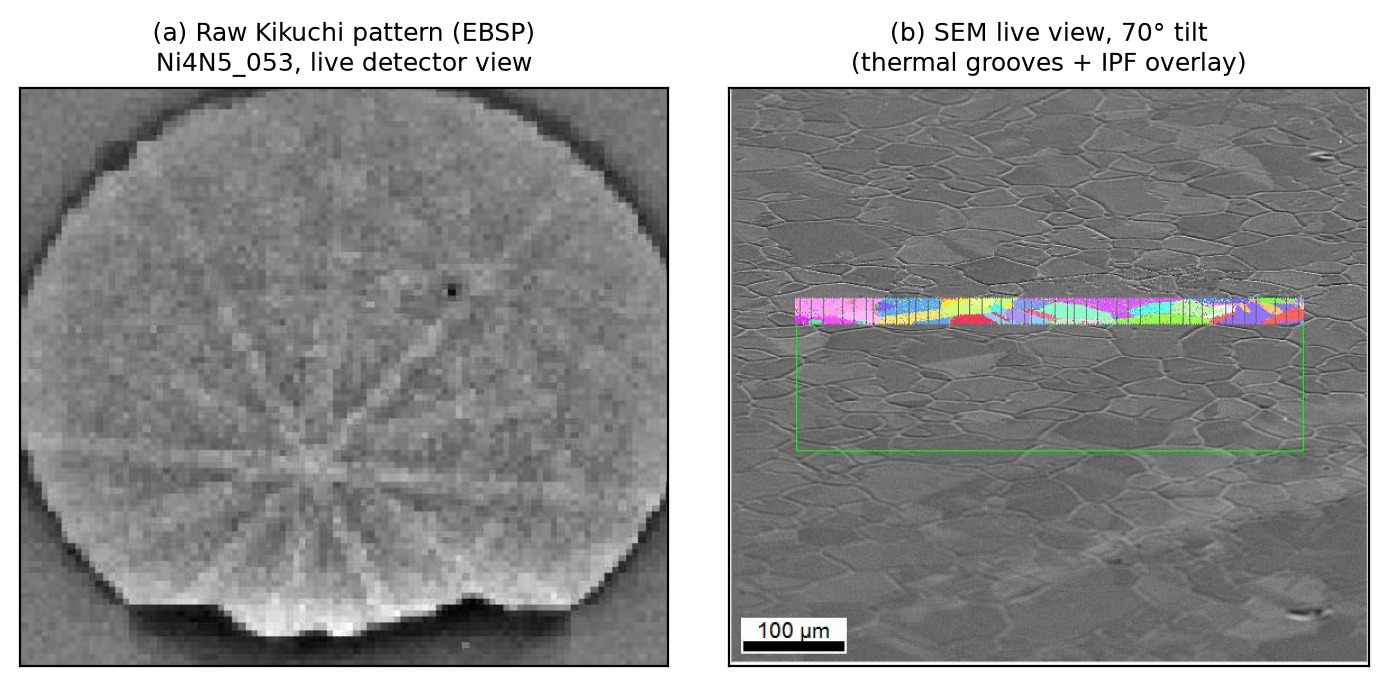
\includegraphics[width=0.8\linewidth]{figures/fig_kikuchi.png}
\caption{Raw (as-collected) EBSD acquisitions from furnace-annealed nickel,
with no metallographic preparation. (a)~Raw Kikuchi pattern (electron
backscatter pattern) of specimen Ni4N5\_028 as seen live on the detector at
$8\times8$ binning (30\,ms exposure), with Kikuchi bands and zone axes
crisply resolved; (b)~the corresponding SEM live view at 70{,}068$\times$,
where thermal grooving alone delineates the grain boundaries crossed by the
EBSD line scans (red marks; 1\um{} scale bar). (c--e)~Representative
per-scan-point raw patterns ($115\times115$\,px at $8\times8$ binning) saved
automatically during EBSD mapping of the early-campaign specimens
Ni\_003b1a and Ni\_003a1b; more than 100{,}000 such patterns are preserved
in the repository's raw-pattern archives
(\texttt{docs/SEM/raw-kikuchi-patterns/}).}
\label{fig:s-kikuchi}
\alttext{Five grayscale panels: a raw Kikuchi diffraction pattern of
intersecting bright bands, an electron micrograph with grooved grain
boundaries and line-scan marks, and three small saved detector patterns.}
\end{figure}

\begin{figure}[htbp]
\centering
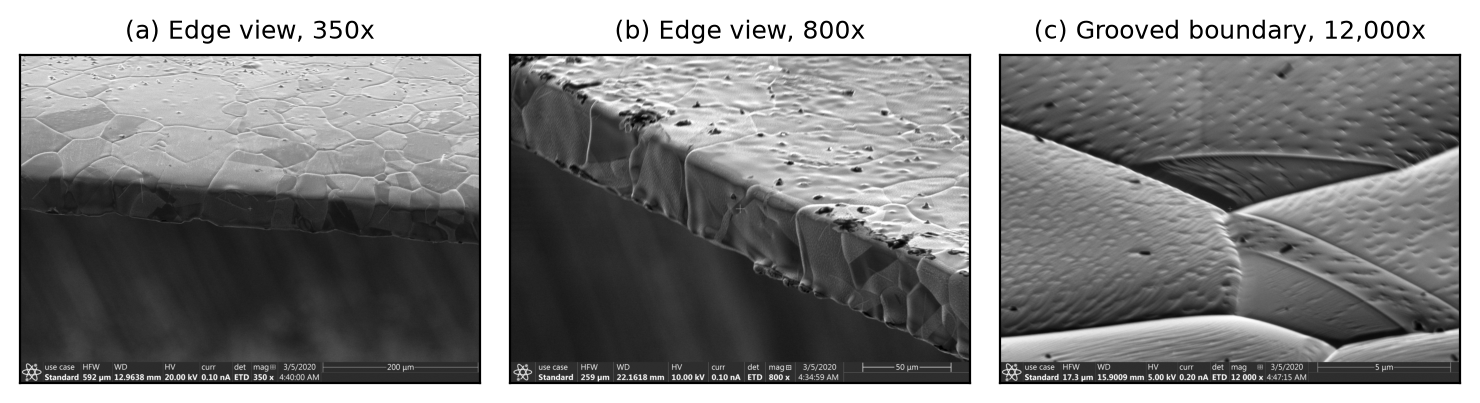
\includegraphics[width=0.8\linewidth]{figures/fig_grooving.png}
\caption{Grain-boundary thermal grooving on specimen Ni4N5\_053 after a
1200\dC{} / 12\,h anneal, imaged edge-on in the as-annealed condition
(ultrasonic ethanol clean only; no polishing). (a)~Edge view at 350$\times$
(200\um{} scale bar): several grain boundaries traverse the full sheet
thickness. (b)~Edge and top surface at 800$\times$ (50\um{} scale bar), with
grooves outlining the surface grain structure. (c)~A single grooved boundary
at 12{,}000$\times$ (5\um{} scale bar): the deep trench develops as
grain-boundary energy equilibrates against surface energy at the soak
temperature.}
\label{fig:s-grooving}
\alttext{Three electron micrographs at increasing magnification showing deep
grooves along grain boundaries on the edge and top surface of an annealed
nickel sheet.}
\end{figure}

\clearpage
%==============================================================
\section{YSZ / high-temperature extension}
%==============================================================

\begin{figure}[htbp]
\centering
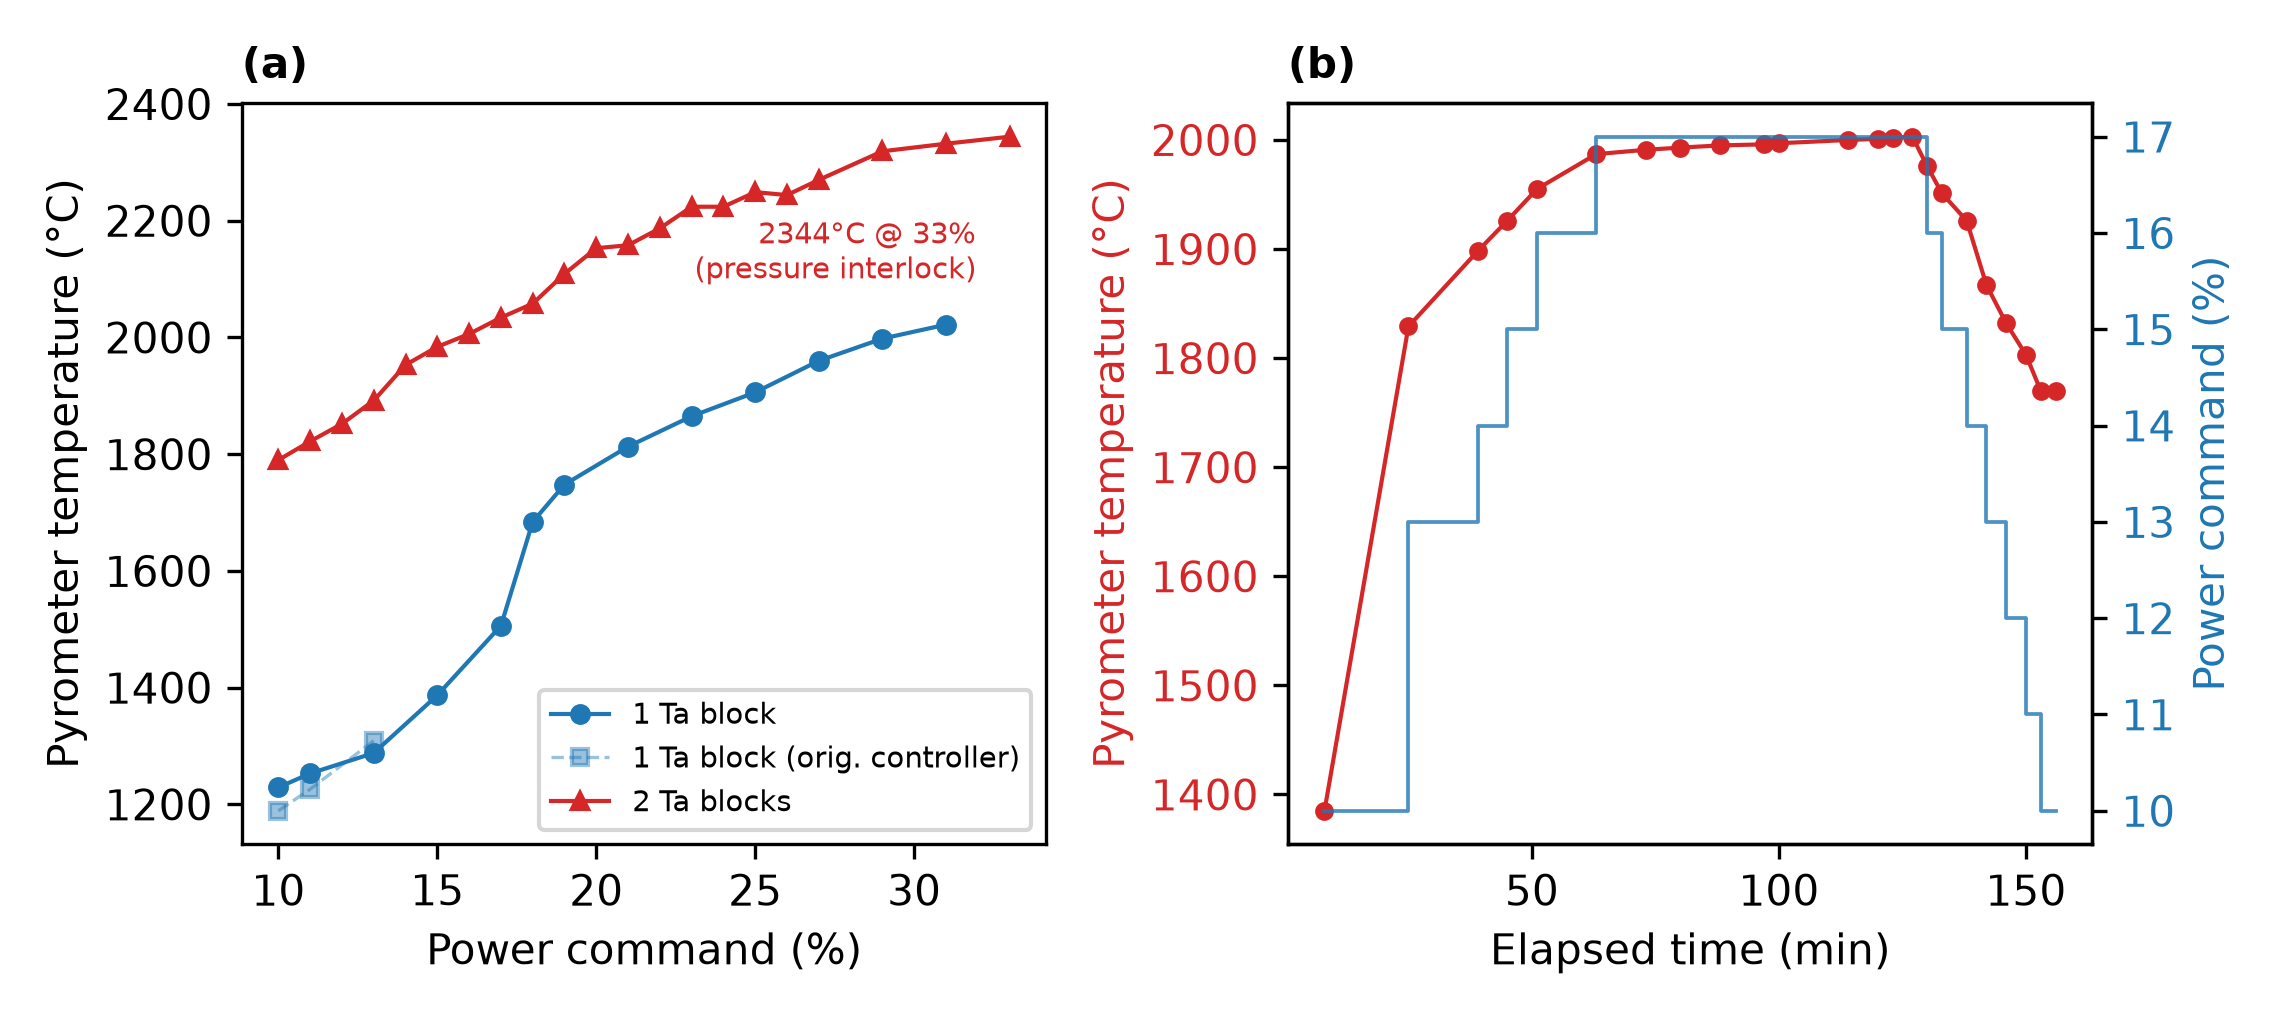
\includegraphics[width=0.78\linewidth]{figures/fig_ta_heatcurve.png}
\caption{Measured heat curves of the tantalum-susceptor (ceramic) stack.
(a)~Pyrometer temperature vs.\ generator power command for one and two
stacked tantalum susceptor blocks (the faint series repeats the single-block
measurement on the original power controller); the two-block ramp reached
2344\dC{} at a 33\,\% command before the chamber pressure interlock ended
the test. (b)~Timed two-block ramp/soak: a constant 17\,\% command holds
$\sim$2000\dC{} ($2000 \pm 3$\dC{} over the final hour) before a stepped
ramp-down.}
\label{fig:s-heatcurve}
\alttext{Two plots: temperature versus power command curves for one and two
tantalum blocks reaching 2344 degrees Celsius, and a timed ramp holding a
steady 2000 degrees Celsius for over an hour.}
\end{figure}

\begin{figure}[htbp]
\centering
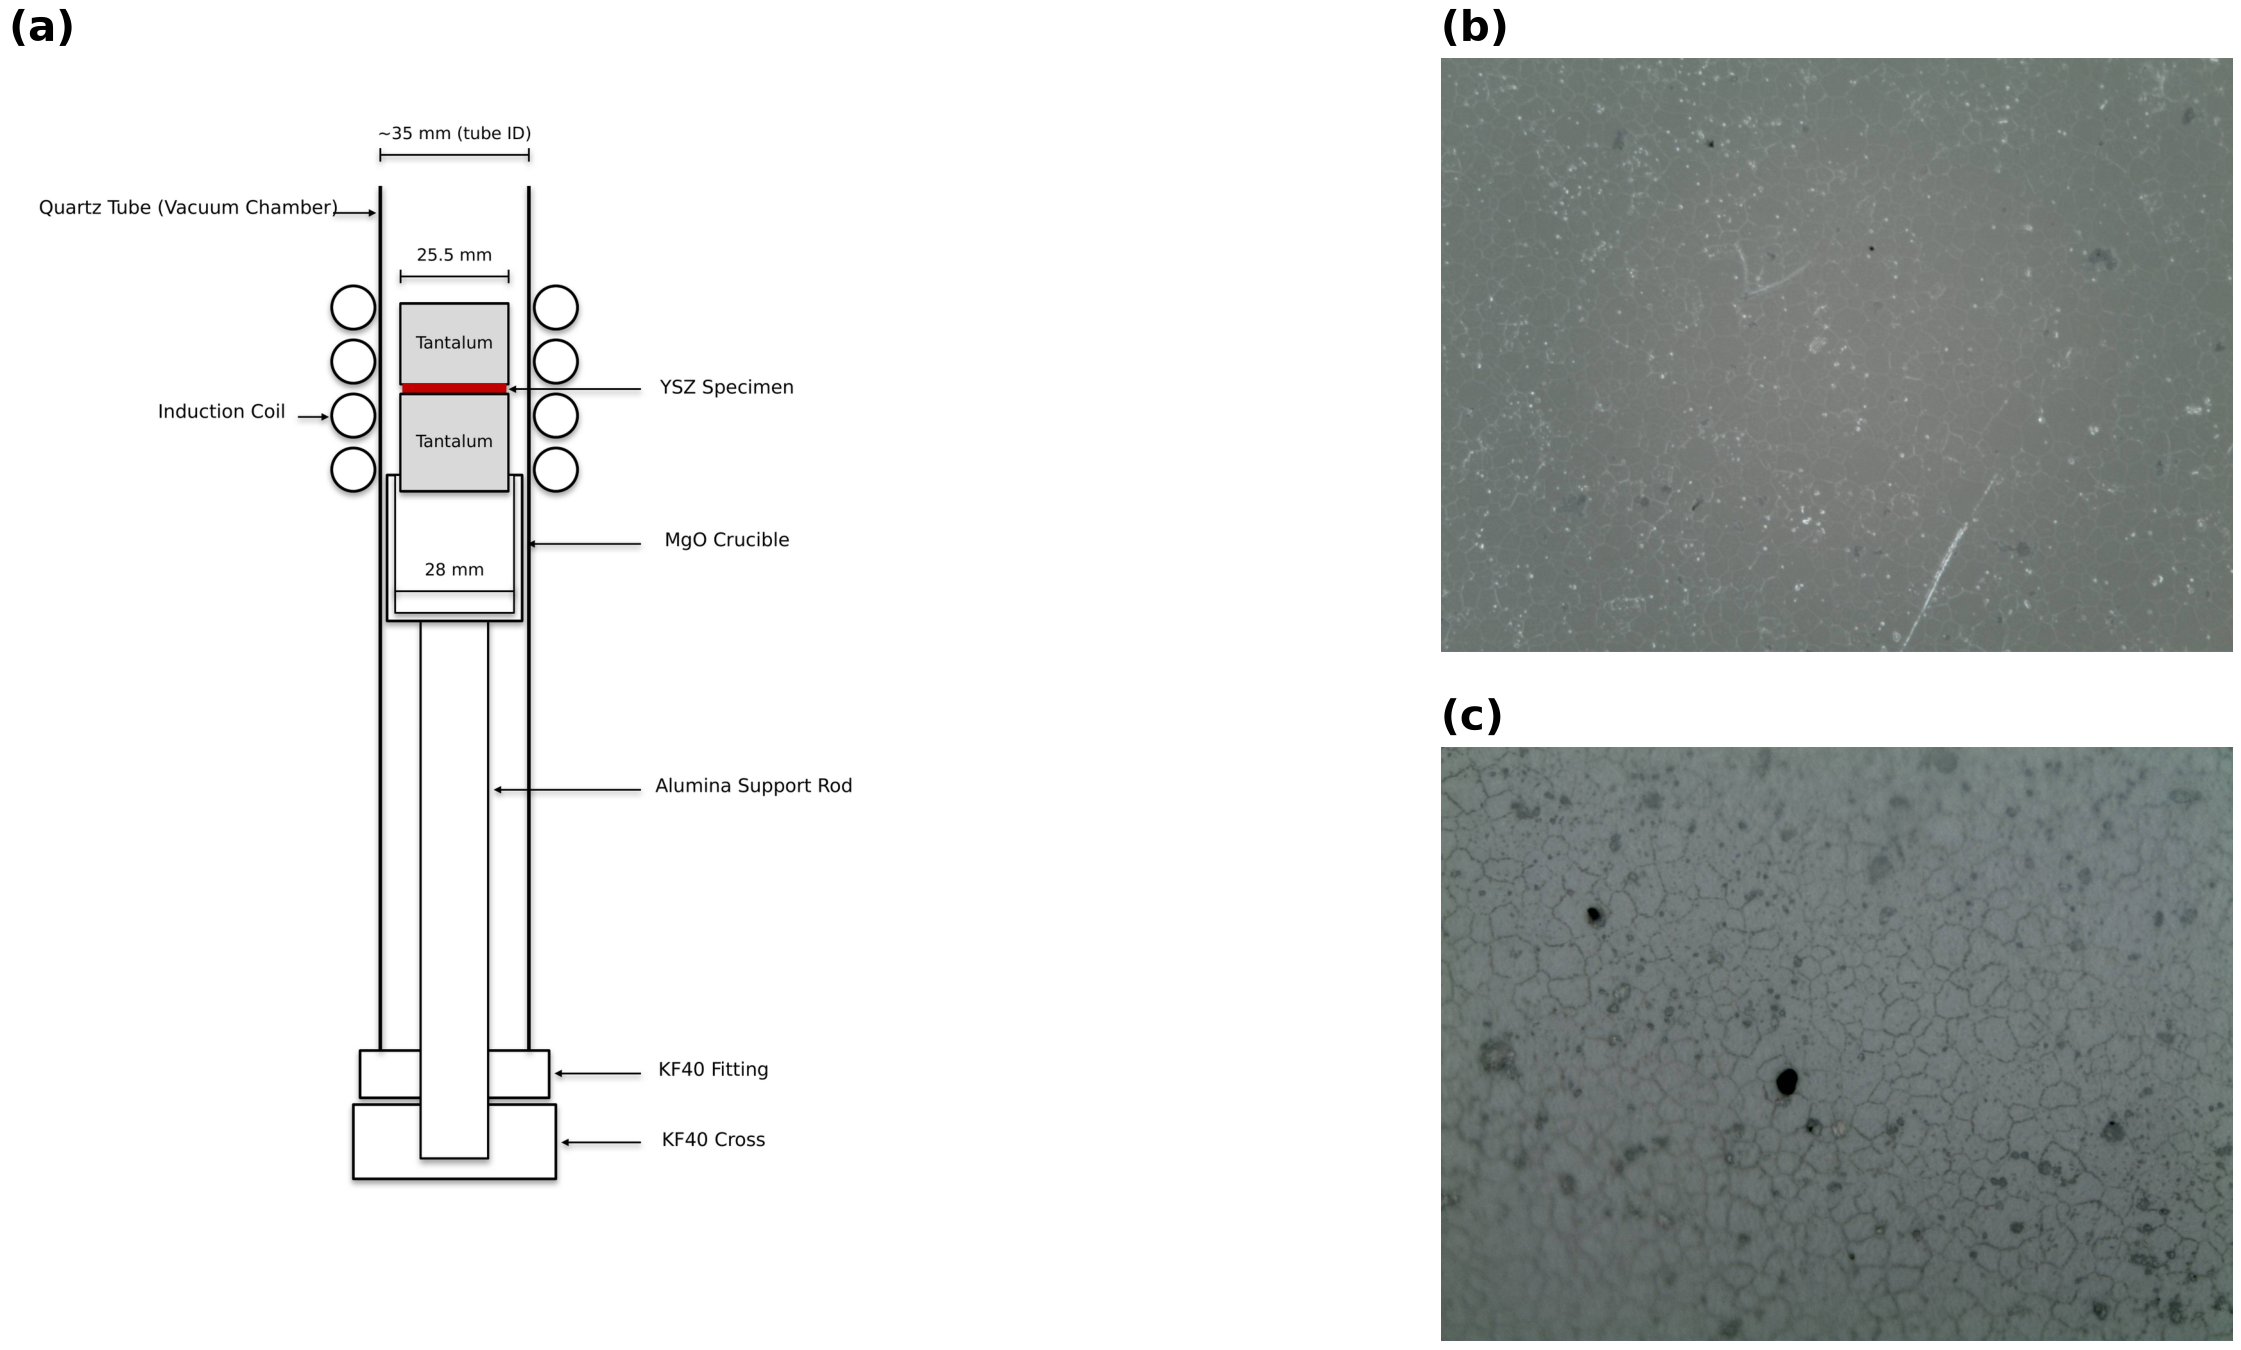
\includegraphics[width=0.85\linewidth]{figures/fig_ysz.png}
\caption{YSZ charge stack and resulting microstructure. (a)~Charge-stack
schematic: inside a fresh $\sim$35\,mm-ID quartz tube, the YSZ specimen
(red) is sandwiched between two 25.5\,mm tantalum susceptor blocks, resting
on a 28\,mm ceramic heat-dissipation stub (boron nitride for best results,
sometimes MgO) on an alumina support rod that raises the stack to coil
height; the coil, vacuum, pyrometer, and control paths are unchanged from
the metal configuration. (b)~Optical micrograph of YSZ after a
1700\dC{} / 10\,h anneal. (c)~Optical micrograph of an induction-annealed
YSZ specimen, showing the equiaxed grain structure.}
\label{fig:s-ysz}
\alttext{A labeled schematic of the tantalum and YSZ charge stack inside a
quartz tube, beside two optical micrographs of equiaxed YSZ grain
structures.}
\end{figure}

\clearpage

%==============================================================
\section{Specimen--thermal-history linkage}
%==============================================================

Table~\ref{tab:linkage} links each characterized specimen to its furnace run
and carries the run-ID-level detail deliberately kept out of the main text.
Each run ID hyperlinks to the raw run log in the data repository. ``Nominal
soak'' is the target parsed from the run filename; ``Logged soak T'' is the
machine-parsed soak-mean from the trace
(\texttt{docs/data\_log/processed/run\_summary.csv}); ``Atmos.''\ indicates
whether active gas flow was present in the parsed log summary, not a fully
reconstructed gas chemistry; ``Characterization'' gives recorded SEM/optical
file counts and flags recorded EBSD/OIM data. Machine-parsed per-run CSV
traces and PNG plots for every linked run are in
\texttt{docs/data\_log/processed/}. The complete 35-specimen
cross-reference, including characterized specimens whose run logs are not in
the parsed set, is \texttt{paper/characterization-crossref.csv} /
\texttt{.md}. Additional raw-pattern context for the Kikuchi figures (main
text Fig.~4 and Fig.~\ref{fig:s-kikuchi}): the live-pattern screenshot of
Ni4N5\_028 is
\texttt{docs/SEM/raw-kikuchi-patterns/200203\_Ni4N5\_028\_s1/Scan3.JPG}, and
the $>$100{,}000 preserved per-scan-point raw patterns of the early-campaign
Ni\_003-series specimens are inventoried in
\texttt{docs/SEM/raw-kikuchi-patterns/README.md}.

\begin{landscape}
\begin{table}[htbp]
\centering
\caption{Specimen\,$\leftrightarrow$\,thermal-history linkage for the runs
used in the manuscript's validation sections. Run IDs link to the raw run
logs in the data repository.}
\label{tab:linkage}
\footnotesize
\setlength{\tabcolsep}{4pt}
\begin{tabular}{llllllll>{\raggedright\arraybackslash}p{3.9cm}}
\toprule
Specimen & Material & Run (raw log) & Nominal soak & Logged soak T & Soak time & Atmos. & Characterization & Role / figure \\
\midrule
Ni4N5\_026 & Ni4N5 & \runlog{IFrun021-040/IFrun039_Ni4N5_026_1200C_6h.xlsx}{IFrun039} & 1200\dC & 1200.4\dC & 6\,h & no-flow & --- & Calibration (Fig.~\ref{fig:s-calibration}) \\
Ni4N5\_027 & Ni4N5 & \runlog{IFrun021-040/IFrun040_Ni4N5_027_1250C_6h.xlsx}{IFrun040} & 1250\dC & 1250.0\dC & 6\,h & no-flow & --- & Calibration \\
Ni4N5\_025 & Ni4N5 & \runlog{IFrun021-040/IFrun038_Ni4N5_025_1300C_1h.xlsx}{IFrun038} & 1300\dC & 1299.9\dC & 1\,h & no-flow & --- & Calibration \\
Ni4N5\_022 & Ni4N5 & \runlog{IFrun021-040/IFrun032_Ni4N5_022_1400C_10min.xlsx}{IFrun032} & 1400\dC & 1399.6\dC & 10\,min & no-flow & --- & Calibration \\
Ni4N5\_084 & Ni4N5 & \runlog{IFrun061-080/IFrun079_Ni4N5_084_1300C_12h.xlsx}{IFrun079} & 1300\dC & 1302.1\dC & 12\,h & flow & --- & Representative soak (Fig.~\ref{fig:s-representative}) \\
Ni4N5\_040 & Ni4N5 & \runlog{IFrun041-060/IFrun052_Ni4N5_040_1200C_12h.xlsx}{IFrun052} & 1200\dC & 1199.8\dC & 12\,h & flow & --- & Repeatability run 1 (Fig.~\ref{fig:s-repeatability}) \\
Ni4N5\_042,044 & Ni4N5 & \runlog{IFrun041-060/IFrun054_Ni4N5_042,044_1200C_12h.xlsx}{IFrun054} & 1200\dC & 1201.5\dC & 12\,h & flow & --- & Repeatability run 2 \\
Ni4N5\_045,046 & Ni4N5 & \runlog{IFrun041-060/IFrun055_Ni4N5_045,046_1200C_12h.xlsx}{IFrun055} & 1200\dC & 1204.2\dC & 12\,h & flow & --- & Repeatability run 3 \\
Ni4N5\_047,048 & Ni4N5 & \runlog{IFrun041-060/IFrun056_Ni4N5_047,048_1200C_12h.xlsx}{IFrun056} & 1200\dC & 1200.6\dC & 12\,h & flow & --- & Repeatability run 4 \\
Ni4N5\_049,050 & Ni4N5 & \runlog{IFrun041-060/IFrun057_Ni4N5_049,050_1200C_12h.xlsx}{IFrun057} & 1200\dC & 1201.2\dC & 12\,h & flow & --- & Repeatability run 5 \\
Ni4N5\_051,052 & Ni4N5 & \runlog{IFrun041-060/IFrun058_Ni4N5_051,052_1200C_12h.xlsx}{IFrun058} & 1200\dC & 1201.0\dC & 12\,h & flow & --- & Repeatability run 6 \\
Ni4N5\_053,054 & Ni4N5 & \runlog{IFrun041-060/IFrun059_Ni4N5_053,054_1200C_12h.xlsx}{IFrun059} & 1200\dC & 1200.3\dC & 12\,h & flow & 4 SEM, 3 opt.\ (Ni4N5\_053) & Repeatability run 7; grooving (Fig.~\ref{fig:s-grooving}) \\
Ni4N5\_056,057 & Ni4N5 & \runlog{IFrun041-060/IFrun060_Ni4N5_056,057_1200C_12h.xlsx}{IFrun060} & 1200\dC & 1200.9\dC & 12\,h & flow & --- & Repeatability run 8 \\
Ni200\_015 & Ni200 & \runlog{IFrun081-100/IFrun081_Ni200_015_1325C_20h.xlsx}{IFrun081} & 1325\dC & 1326.5\dC & 20\,h & flow & 3 opt. & Long soak, 20\,h (Fig.~\ref{fig:s-longsoak}) \\
Ni200\_017 & Ni200 & \runlog{IFrun061-080/IFrun080_Ni200_017_1325C_40h.xlsx}{IFrun080} & 1325\dC & 1326.3\dC & 40\,h & flow & 2 opt. & Long soak, 40\,h (Fig.~\ref{fig:s-longsoak}) \\
Ni4N5\_079,080 & Ni4N5 & \runlog{IFrun061-080/IFrun072_Ni4N5_079,080_1400C_12h.xlsx}{IFrun072} & 1400\dC & --- & 12\,h & flow & --- & Process-window specimen \\
Ni4N5\_034 & Ni4N5 & \runlog{IFrun041-060/IFrun049_Ni4N5_034_1200C_12h.xlsx}{IFrun049} & 1200\dC & 1200.0\dC & 12\,h & no-flow & 4 SEM, EBSD & EBSD IPF map (Fig.~\ref{fig:s-ebsd}a) \\
Ni4N5\_081 & Ni4N5 & \runlog{IFrun081-100/IFrun082_Ni4N5_081_1300C_20h.xlsx}{IFrun082} & 1300\dC & 1301.4\dC & 20\,h & flow & 10 SEM, 10 opt., EBSD & Microstructure (main text Fig.~5) \\
Ni4N5\_010 & Ni4N5 & \runlog{IFrun001-020/IFrun016_Ni4N5_010.xlsx}{IFrun016} & 1200\dC & 1199.9\dC & --- & no-flow & 4 opt. & Characterization only \\
Ni4N5\_012 & Ni4N5 & \runlog{IFrun001-020/IFrun019_Ni4N5_012.xlsx}{IFrun019} & 1200\dC & 1199.6\dC & --- & no-flow & 1 opt. & Characterization only \\
Ni200\_001 & Ni200 & \runlog{IFrun001-020/Ni200_001_IFrun004.lvm}{IFrun004}/\runlog{IFrun001-020/Ni200_001_IFrun005.lvm}{IFrun005} & --- & --- & --- & no-flow & 3 opt. & Characterization only \\
Ni4N5\_001b & Ni4N5 & IFrun006 (log not in parsed set) & --- & --- & --- & no-flow & 2 opt. & Characterization only \\
\bottomrule
\end{tabular}
\alttext{Table linking each specimen to its furnace run, nominal and logged
soak temperature, soak time, atmosphere, characterization file counts, and
its role or figure in the manuscript.}
\end{table}
\end{landscape}

\clearpage
%==============================================================
\section{Bill of materials}
%==============================================================

Table~\ref{tab:bom} is the itemized bill of materials for the reproducible
build; the main text's Construction section cites the package-level cost and
points here. Groupings by designator prefix: GEN = induction generator
package (generator, controller, chiller, heating head, line transformer),
RETRO = the reproducible retrofit (control / vacuum / sensing) parts, CONS =
consumables. Full vendor/price detail for the RETRO and CONS parts is in
\texttt{paper/extracted-context/parts\_list.md} (extracted from
\texttt{docs/induction\_parts\_list.xlsx}). All costs are in USD; prices are
the laboratory's purchase records (quote years 2019--2021), several from
used/surplus sources as noted; shipping and tax are excluded unless stated.
The GEN line items are from a single vendor quote (generator, heating head,
controller, chiller, and line transformer totaling \$16{,}487). For the
high-temperature ceramic (YSZ) configuration, the graphite crucible stack is
exchanged for tantalum susceptor blocks resting on a ceramic
heat-dissipation stub (boron nitride for best results, sometimes MgO);
vendor records for the tantalum blocks and BN stubs are not in the archived
parts list.

\begin{table}[htbp]
\centering
\caption{Itemized bill of materials for the reproducible build (USD).}
\label{tab:bom}
\footnotesize
\setlength{\tabcolsep}{4pt}
\begin{tabular}{lL{5.4cm}cL{1.8cm}L{1.4cm}L{3.1cm}L{1.3cm}}
\toprule
Desig. & Component & No. & Unit \$ & Total & Source & Material \\
\midrule
GEN-1 & CEIA ``Power Cube'' PW3-90/50 solid-state RF generator (V3000-0070) & 1 & \$8{,}240 & \$8{,}240 & East Coast Induction (USA) & --- \\
GEN-2 & Power Controller C-V3 Plus (V3000-0414) & 1 & \$1{,}670 & \$1{,}670 & East Coast Induction (USA) & --- \\
GEN-3 & Recirculating chiller (MIL043008 air-cooled closed-loop, V1650-0060; vendor-listed as a water chiller, but the loop is charged with ethylene glycol coolant) & 1 & \$1{,}575 & \$1{,}575 & East Coast Induction (USA) & --- \\
GEN-4 & Heating head + 3\,m cable and coolant lines (PWH-13-12-30/50, V3000-0300); 1 coil made to spec at no charge with a complete unit & 1 & \$3{,}337 & \$3{,}337 & East Coast Induction (USA) & copper \\
GEN-5 & Line auto-transformer, 12\,kVA / 3PH / 480$\times$380\,V with taps (V049-0508; facility-dependent) & 1 & \$1{,}665 & \$1{,}665 & East Coast Induction (USA) & --- \\
RETRO-1 & LabVIEW-compatible DAQ with analog out + in (0--5\,V AO): NI USB-6000 DAQ & 1 & \$281.00 & \$281.00 & National Instruments & --- \\
RETRO-2 & Dual-wavelength ratio pyrometer (LumaSense IMPAC ISR~6, 800--2500\dC), used & 1 & \$385.00 (used) & \$385.00 & eBay --- used listing (new list $\sim$\$5{,}500, LumaSense quote 00161403) & --- \\
RETRO-3 & 24\,V linear power supply for pyrometer (International Power) & 1 & \$51 & \$51 & Mouser & --- \\
RETRO-4 & Voltage-to-current (0--5\,V $\rightarrow$ 4--20\,mA) loop conditioner set for generator power-setpoint input (NI-9265 input module + NI-9203 output module + NI cDAQ-9174 chassis) & 1 set & \$3{,}755.00 & \$3{,}755.00 & National Instruments & --- \\
RETRO-5 & Edwards nEXT T-Station 85H Dry turbo pumping station (1Ph 100--120\,V, 50/60\,Hz, DN 40 ISO-KF) & 1 & \$13{,}573.65 & \$13{,}573.65 & Edwards Vacuum & --- \\
RETRO-5A & Wide-range vacuum gauge D14701000 (36\,V, 2\,W); discontinued, replaced by D3G0021100 & 1 & \$1{,}543.29 & \$1{,}543.29 & Chemtech Scientific & --- \\
RETRO-6 & Edwards TAV5 vent valve (new) & 1 & \$652.80 & \$652.80 & Edwards Vacuum & --- \\
RETRO-6A & Sierra SmartTrak 100L mass flow controller (optional; helpful when continuous inert gas flow is required) & 1 & \$550--\$1{,}000 (quote range) & \$550--\$1{,}000 & Sierra / distributor quote & --- \\
RETRO-7 & Inert-gas regulator (Fisher FS-50) & 1 & \$38 & \$38 & Fisher Scientific & --- \\
RETRO-8 & KF40 overpressure centering ring & 1 & \$19 & \$19 & IdealVac & aluminum \\
RETRO-9 & KF40 plastic quick vacuum clamp & 1 & \$23 & \$23 & IdealVac & polymer \\
RETRO-10 & Optical window, custom quartz disc 55\,mm $\times$ 1.5\,mm (1 used; buy 3 for spares) & 3 & \$18 (est.) & \$54 & Custom-cut metric disc --- vendor not recorded in parts list; price approximate (McMaster stocks only imperial sizes) & fused quartz \\
RETRO-11 & Ultra-high-temperature quartz disc 2\,in $\times$ 1/16\,in (McMaster 1357T12) & 1 & \$19 & \$19 & McMaster-Carr & fused quartz \\
RETRO-12 & Inert-gas plumbing (BSPT/KF adapters, barbs, tee, 10\,psi relief valve McMaster 4772K4) & 1 set & see parts list & $\sim$\$66 & McMaster-Carr / BMotionTech & brass / steel \\
CONS-1 & Quartz tube, 4\,ft $\times$ 35\,mm ID, cut to length & 2 & \$67 & \$134 & QSI Quartz & fused quartz \\
CONS-2 & Graphite stock for machined crucible/susceptor (56L-3, 3000\dC, 1$\times$6$\times$6\,in) & 1 & \$99 & \$99 & Cotronics & graphite \\
CONS-3 & Graphite repair cement (Resbond 931-1, 3000\dC) & 1 & \$108 & \$108 & Cotronics & graphite \\
CONS-4 & Alumina crucible stock (RTC-60-2, 1787\dC, 10\,lb) & 1 & \$91 & \$91 & Cotronics & alumina \\
CONS-5 & Zirconia crucible stock (760-1, 2204\dC, 10\,lb) & 1 & \$124 & \$124 & Cotronics & zirconia \\
CONS-6 & Torr-Seal high-vacuum epoxy / O-rings & 1 set & \$57 & \$57 & Varian / McMaster & epoxy / elastomer \\
\bottomrule
\end{tabular}
\alttext{Itemized bill of materials with designator, component description,
quantity, unit and total cost in US dollars, source, and material for each
generator, retrofit, and consumable part.}
\end{table}

\clearpage

%==============================================================
\section{Design-file inventory}
%==============================================================

Table~\ref{tab:designfiles} lists the open design files in the repository
(paths relative to the repository root; the archival snapshot is the Zenodo
deposit above). The graphite crucible/susceptor machining drawing is
pending; its measured dimensions are given in
Fig.~\ref{fig:s-crucible-dims}. Exports of the LabVIEW block diagrams to
PDF/PNG for non-LabVIEW readers are likewise pending.

\begin{table}[htbp]
\centering
\caption{Open design files in the repository.}
\label{tab:designfiles}
\footnotesize
\begin{tabular}{L{5.6cm}L{2.6cm}L{2.6cm}L{4.6cm}}
\toprule
Design file & File type & License & Location \\
\midrule
LabVIEW control VIs (furnace control, manual control, PID tuning v1/v2, email alert) & LabVIEW \texttt{.vi} & MIT (proposed) & \path{code/induction-furnace-control-code/} \\
Manual ramping v5 VIs & LabVIEW \texttt{.vi} & MIT (proposed) & \texttt{code/manual-ramping-v5/} \\
\texttt{plotheatcurve.m} (heat-curve plotter) & MATLAB & MIT (proposed) & \texttt{code/plotheatcurve.m} \\
Work-coil drawing & PDF / OXPS & CERN-OHL-S (proposed) & \texttt{docs/coils-drawing.pdf}, \texttt{docs/coils.oxps} \\
System schematics & PPTX (+ extracted text/figures) & CERN-OHL-S (proposed) & \texttt{docs/*.pptx}, \path{paper/extracted-context/} \\
Temperature-control wiring & PNG & CERN-OHL-S (proposed) & \path{docs/temp-control-modification/} \\
KF40 overpressure centering ring & STEP & CERN-OHL-S (proposed) & \texttt{docs/KF Supplies/} \\
YSZ / tantalum-susceptor stack: schematic, heat-curve workbook, configuration survey, compatibility notes & PNG / XLSX / PDF / DOCX & CERN-OHL-S (proposed) & \texttt{docs/YSZ/} \\
Graphite crucible/susceptor machining drawing & pending & CERN-OHL-S (proposed) & pending (dimensions in Fig.~\ref{fig:s-crucible-dims}) \\
\bottomrule
\end{tabular}
\alttext{Table listing each open design file, its file type, proposed
license, and its location in the repository.}
\end{table}

\end{document}
